\subsection{Lexical Analysis}
The scanner \ref{sec:scannertheory} is the first part of the \textit{lexical analysis}, the scanner divides the source code, according to the Action Grammar found in appendix \ref{actiongrammar}.\\
The scanner can best be described as an automaton \ref{pic:action_atomaton}, which accepts any combination of the terminal symbols defined as letters or digits, a number, or any keyword from the Action Grammar.\\
As an example would the phrase "12 move up", be analyzed as a combination of three tokens.\\

\begin{figure}[h]
\begin{center}
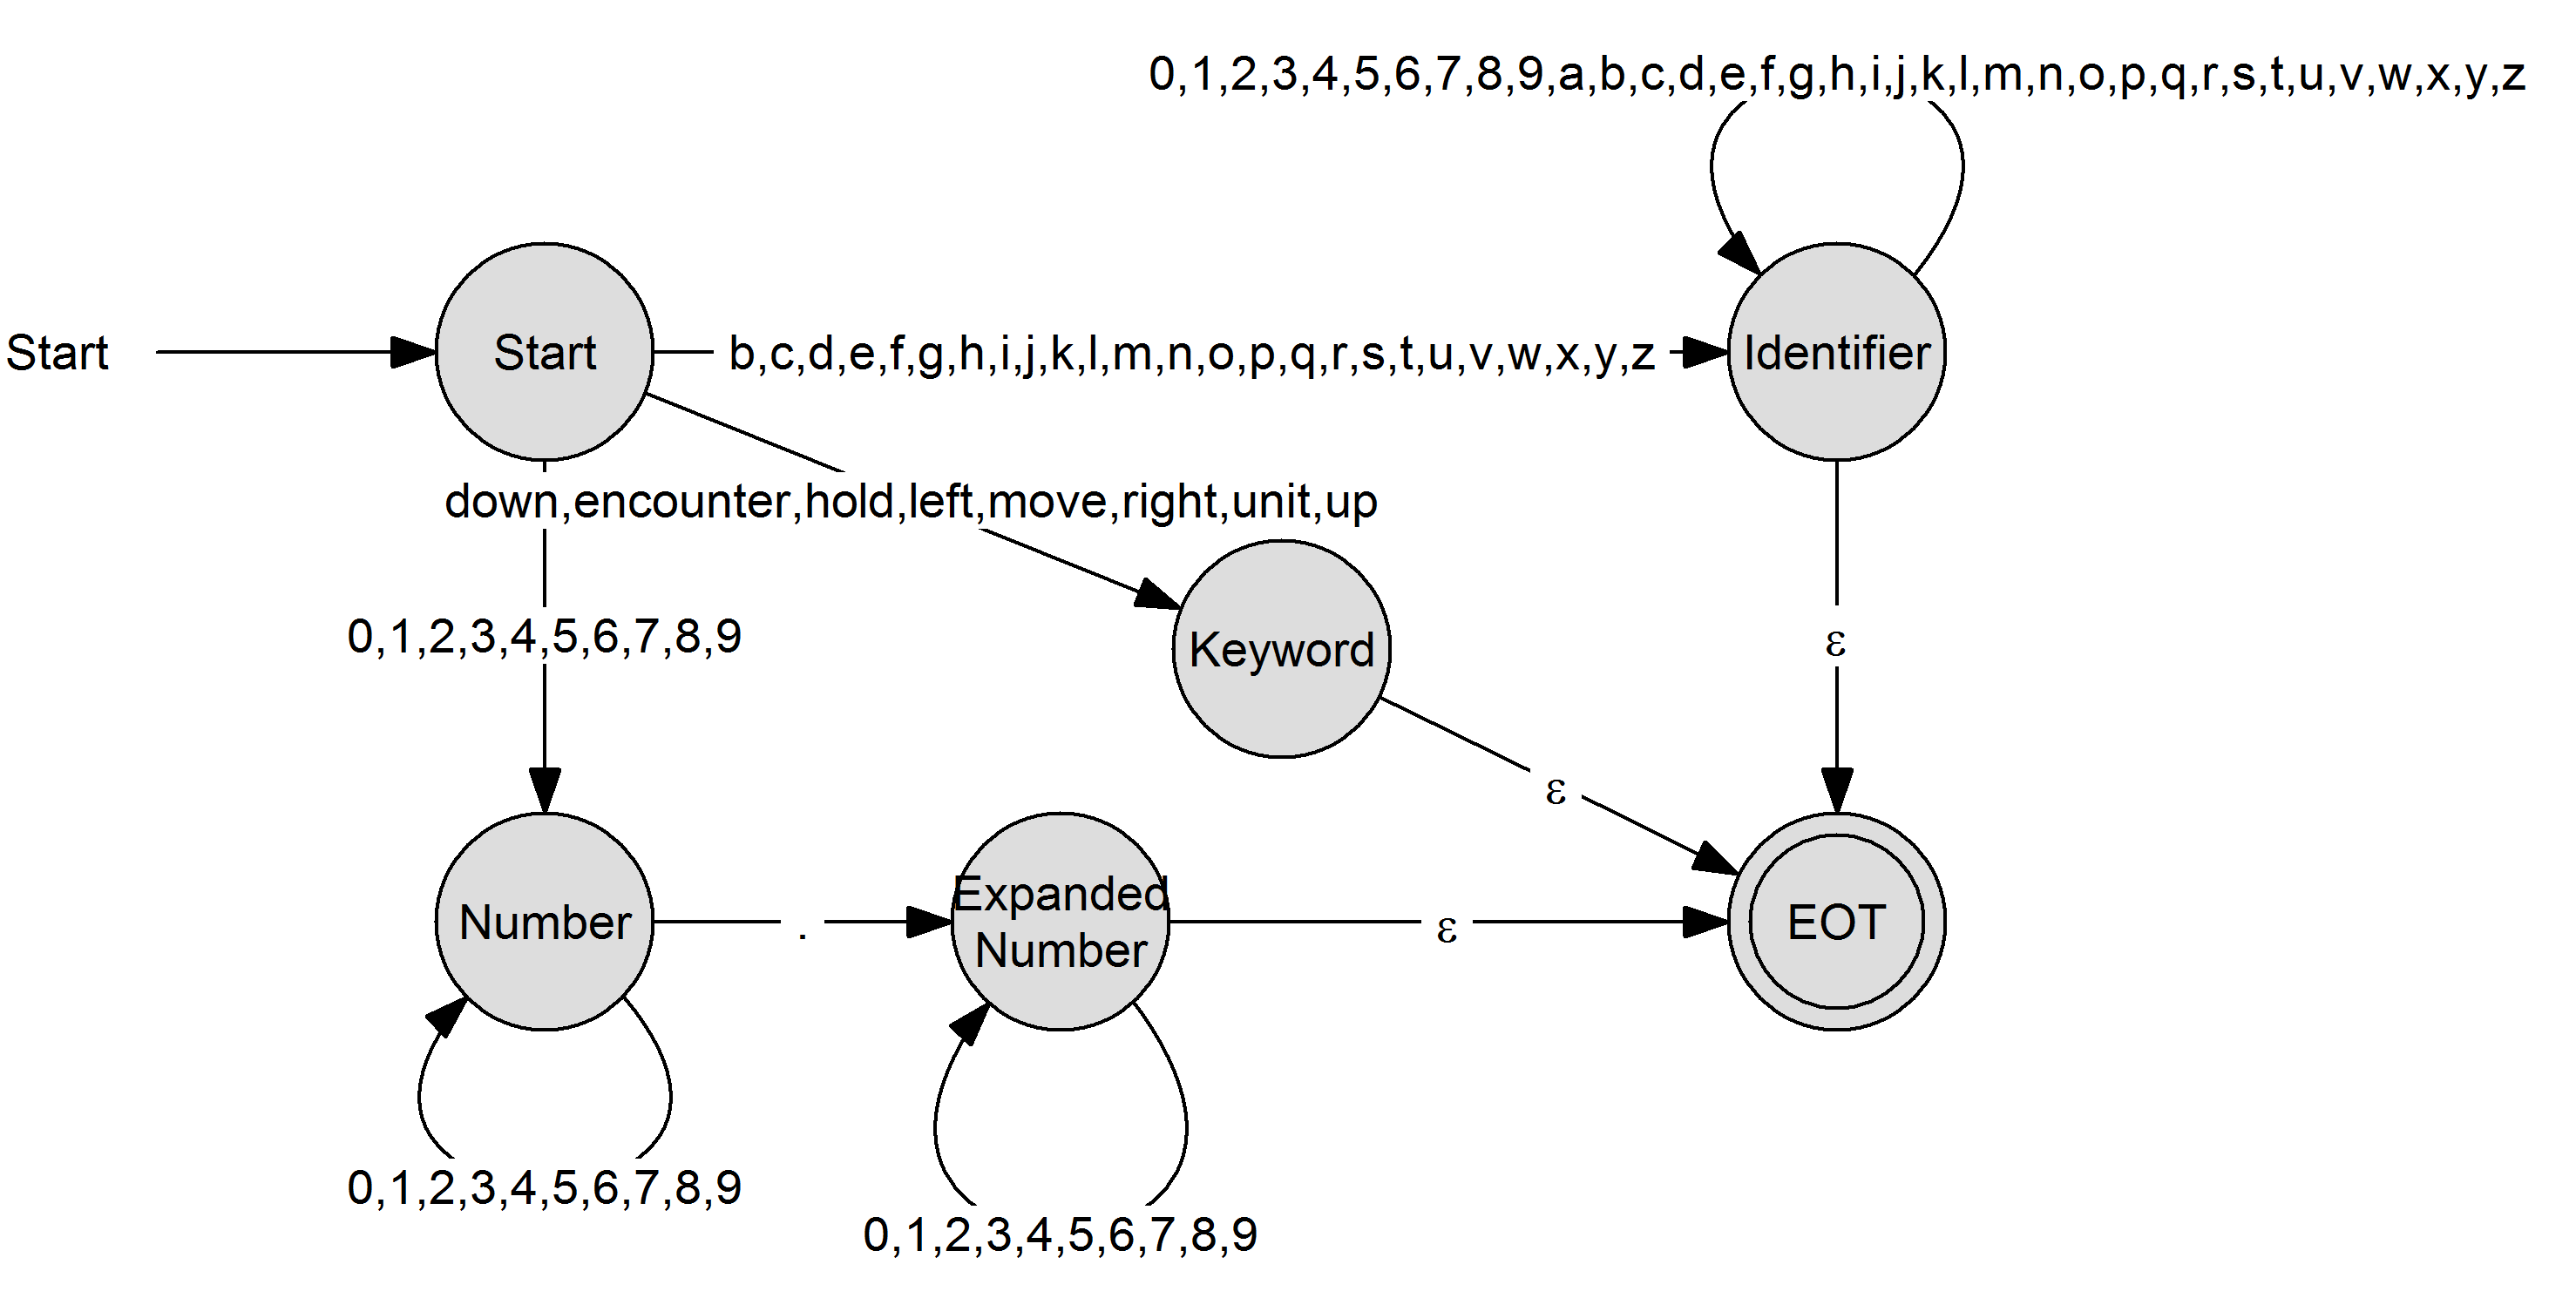
\includegraphics[scale=0.15]{Images/actioninterpreter/ai_automaton.png}
\caption{Atomaton of the Action Interpreters language.}
\label{pic:action_atomaton}
\end{center}
\end{figure}

These three tokens are stored in a list containing all tokens the scanner finds. Since this is an interpreter the scanner only analyse one command at the time.\\
Therefor the AST returned by the parser is really simple, the AST created from the tokens recieved by the scanner  can look like \ref{pic:ai_parser_ast}.

\begin{figure}[h]
\begin{center}
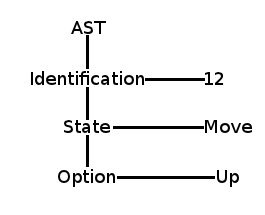
\includegraphics[scale=0.5]{Images/actioninterpreter/AST.png}
\end{center}
\caption{The AST parse from the stream of tokens recieved by the scanner.}
\label{pic:ai_parser_ast}
\end{figure}

The parser is overall pretty simple, since the majority of the parser is the three switches, identification, state, and option. An example of a switch is the identification of the identifier, which parses the first part of the command.\\
SquadID and agentID, has an equivilent TeamID and SquadID, these classes are placeholders used by the visitor to determine which kind of identifier it is when decorating.

\begin{source}{Example of how the parser identifies the identifier.}{}
case (int)Token.keywords.SQUAD:
case (int)Token.keywords.S:
	// Accepts the token, since its either S or Squad.
   	acceptIt();
    squadID squad = parseSquadID();
    return squad;
case (int)Token.keywords.NUMBER:
	// If only a number has been selected, parse it as an Agent ID.
	agentID agentNum = parseagentID();
    return agentNum;
case (int)Token.keywords.IDENTIFIER:
    // If the identification is an identifier, treat it as one.
    Identifier ident = parseIdentifier();
	return ident;
\end{source}